

\tikzset{every picture/.style={line width=0.75pt}} %set default line width to 0.75pt        

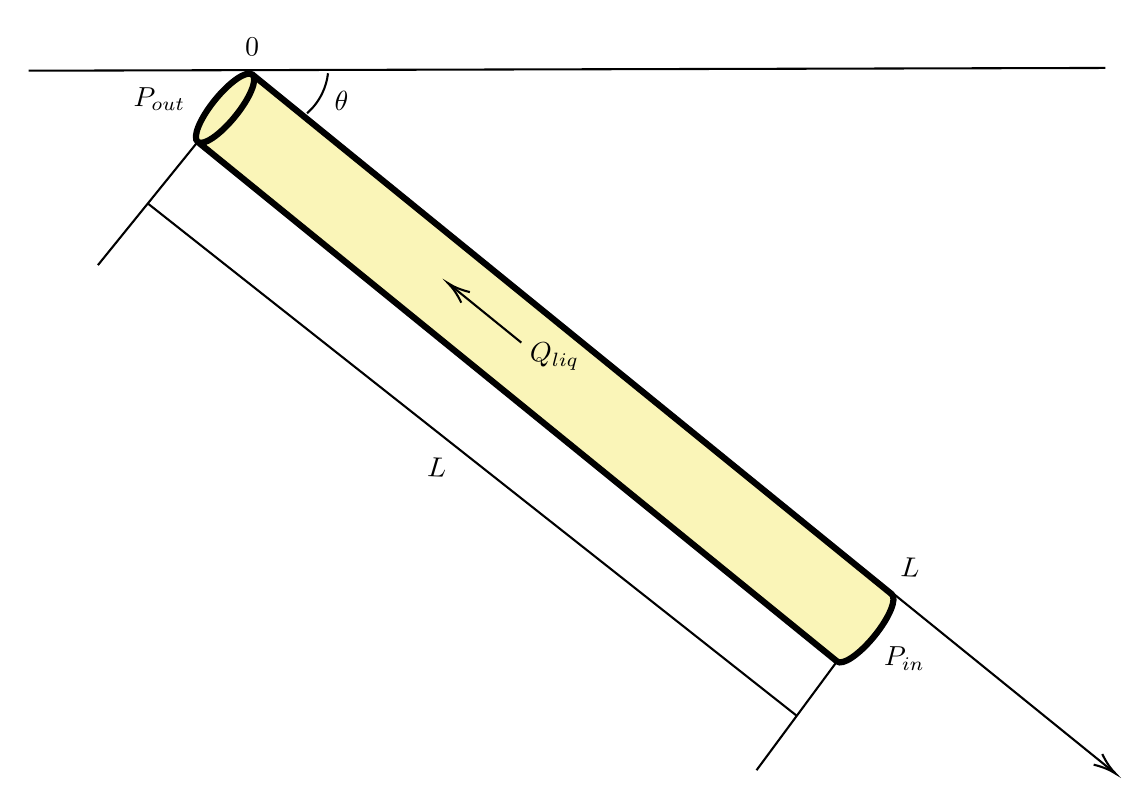
\begin{tikzpicture}[x=0.75pt,y=0.75pt,yscale=-1,xscale=1]
%uncomment if require: \path (0,395); %set diagram left start at 0, and has height of 395

%Shape: Can [id:dp21085002105230832] 
\draw  [fill={rgb, 255:red, 250; green, 245; blue, 184 }  ,fill opacity=1 ][line width=2.25]  (210.09,26.86) -- (518.1,277.18) .. controls (520.79,279.36) and (517.07,288.39) .. (509.8,297.34) .. controls (502.52,306.29) and (494.45,311.77) .. (491.76,309.59) -- (183.75,59.28) .. controls (181.07,57.09) and (184.79,48.07) .. (192.06,39.12) .. controls (199.33,30.17) and (207.41,24.68) .. (210.09,26.86) .. controls (212.78,29.05) and (209.06,38.07) .. (201.78,47.02) .. controls (194.51,55.97) and (186.44,61.46) .. (183.75,59.28) ;
%Shape: Arc [id:dp4551319717308462] 
\draw  [draw opacity=0] (246.53,26.24) .. controls (246.15,29.58) and (245.2,32.91) .. (243.64,36.1) .. controls (241.82,39.8) and (239.34,42.95) .. (236.42,45.5) -- (216.71,22.87) -- cycle ; \draw   (246.53,26.24) .. controls (246.15,29.58) and (245.2,32.91) .. (243.64,36.1) .. controls (241.82,39.8) and (239.34,42.95) .. (236.42,45.5) ;
%Straight Lines [id:da16470020046137734] 
\draw    (183.75,59.28) -- (135.67,118.67) ;
%Straight Lines [id:da017961424869073594] 
\draw    (491.76,309.59) -- (453,362) ;
%Straight Lines [id:da6308247520600512] 
\draw    (159.71,88.97) -- (472.38,335.8) ;
%Straight Lines [id:da6626067218684242] 
\draw    (339.67,156) -- (305.89,128.6) ;
\draw [shift={(304.33,127.34)}, rotate = 399.05] [color={rgb, 255:red, 0; green, 0; blue, 0 }  ][line width=0.75]    (10.93,-3.29) .. controls (6.95,-1.4) and (3.31,-0.3) .. (0,0) .. controls (3.31,0.3) and (6.95,1.4) .. (10.93,3.29)   ;
%Straight Lines [id:da9499771576021536] 
\draw    (102.33,25) -- (621,23.67) ;
%Straight Lines [id:da9922530196016488] 
\draw    (210.09,26.86) -- (624.45,362.41) ;
\draw [shift={(626,363.67)}, rotate = 219] [color={rgb, 255:red, 0; green, 0; blue, 0 }  ][line width=0.75]    (10.93,-3.29) .. controls (6.95,-1.4) and (3.31,-0.3) .. (0,0) .. controls (3.31,0.3) and (6.95,1.4) .. (10.93,3.29)   ;

% Text Node
\draw (253,39.67) node    {$\theta $};
% Text Node
\draw (299,216.33) node  [rotate=-2.44]  {$L$};
% Text Node
\draw (524.33,308.33) node  [rotate=-0.74]  {$P_{in}$};
% Text Node
\draw (165.33,38.67) node  [rotate=-0.74]  {$P_{out}$};
% Text Node
\draw (355.67,162.67) node  [rotate=-0.61]  {$Q_{liq}$};
% Text Node
\draw (210,13.33) node  [rotate=-2.44]  {$0$};
% Text Node
\draw (527,264.33) node  [rotate=-2.44]  {$L$};


\end{tikzpicture}